%\documentclass[aspectratio=43]{beamer}
%\documentclass[aspectratio=1610]{beamer}
\documentclass[aspectratio=169]{beamer}

% @IMP@ \usepackage{pgfpages}
% @IMP@ \pgfpagesuselayout{2 on 1}[a4paper,border shrink=5mm]

\usepackage{fixltx2e}

\usepackage[english,french]{babel}
\usepackage[T1]{fontenc}
\usepackage[utf8]{inputenc}
\usepackage{microtype}

\usepackage{lmodern}

\usepackage{amsmath}
\usepackage{array}
\usepackage{bookmark}
\usepackage{graphicx}
\usepackage{keystroke}
\usepackage{marvosym}
\usepackage{siunitx}
\usepackage{tabularx}
\usepackage{tabulary}
\usepackage{tikz}
\usepackage{xspace}

\usepackage{formation}

% beamer

%\usetheme[formation]{Linagora}
\usetheme{metropolis}

\title{PostgreSQL}
\subtitle{DBA Infrastructure}

%\setbeameroption{show notes}

% array

\setlength{\extrarowheight}{2pt}

% babel

\frenchbsetup{og=«,fg=»}

\newcommand{\anglais}[1]{\textit{\foreignlanguage{english}{#1}}}

% graphicx

\graphicspath{{illustrations/}}

% marvosym

\newcommand{\curseur}{\Rectsteel}

% siunitx

\sisetup
{
	binary-units	= true ,
}

\DeclareSIUnit{\octet}{o}

% tikz

\usetikzlibrary{calc,decorations.pathmorphing}

%%%%%%%%%%%%%%%%%%%%%%%%%%%%%%%%%%%%%%%%%%%%%%%%%%%%%%%%%%%%%%%%%%%%%%%%%%%%%%%%

\begin{document}

%%%%%%%%%%%%%%%%%%%%%%%%%%%%%%%%%%%%%%%%%%%%%%%%%%%%%%%%%%%%%%%%%%%%%%%%%%%%%%%%

\begin{frame}

\pdfbookmark[2]{\inserttitle\ -- \insertsubtitle}{titre}

\titlepage

\end{frame}

%%%%%%%%%%%%%%%%%%%%%%%%%%%%%%%%%%%%%%%%%%%%%%%%%%%%%%%%%%%%%%%%%%%%%%%%%%%%%%%%

\section*{Introduction}

\pdfbookmark[2]{Introduction}{introduction}

%%%%%%%%%%%%%%%%%%%%%%%%%%%%%%%%%%%%%%%%%%%%%%%%%%%%%%%%%%%%%%%%%%%%%%%%%%%%%%%%

\section{PostgreSQL Internals}

%%%%%%%%%%%%%%%%%%%%%%%%%%%%%%%%%%%%%%%%%%%%%%%%%%%%%%%%%%%%%%%%%%%%%%%%%%%%%%%%

\subsection{Point in Time Recovery}

%%%%%%%%%%%%%%%%%%%%%%%%%%%%%%%%%%%%%%%%%%%%%%%%%%%%%%%%%%%%%%%%%%%%%%%%%%%%%%%%

\begin{frame}{Cycle des données dans PostgreSQL}

\begin{figure}
\begin{center}
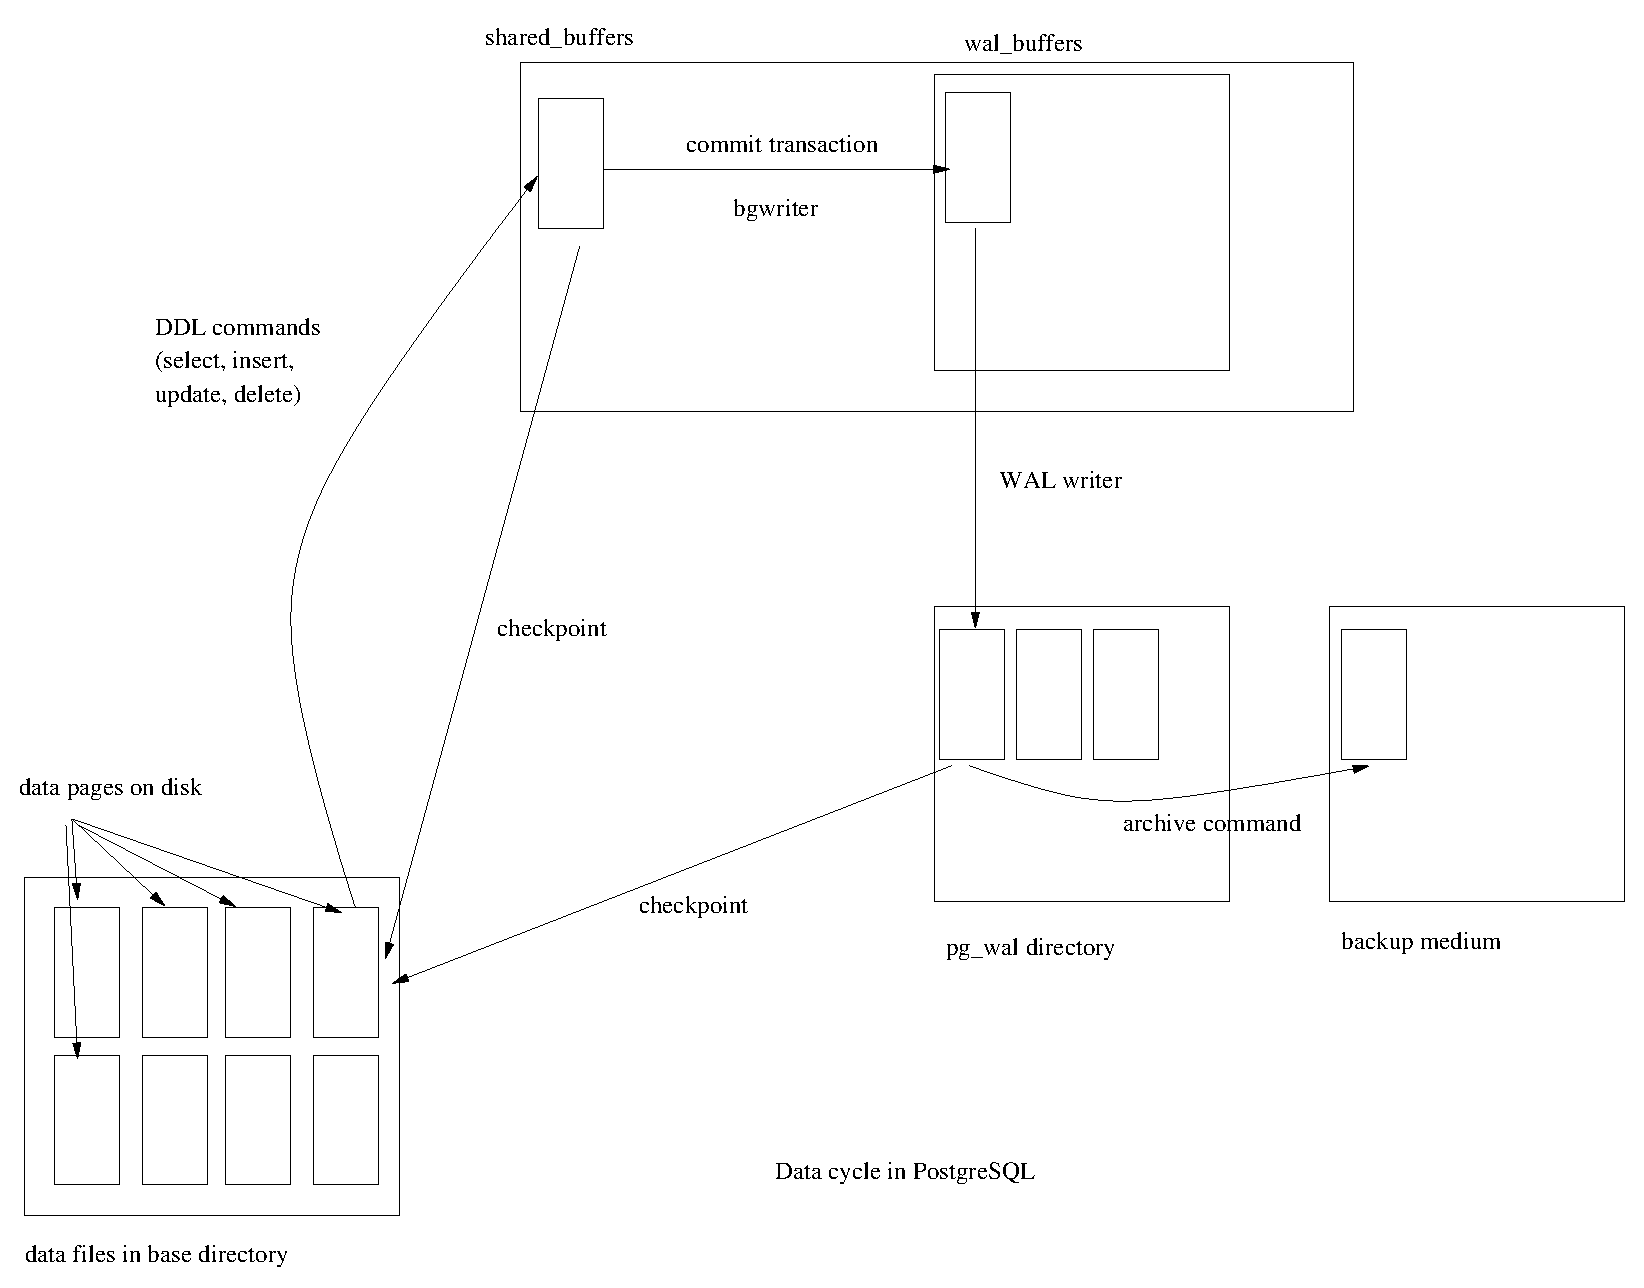
\includegraphics[angle=0, width=0.5\textwidth]{images/internals.eps}
\end{center}
\end{figure}

\begin{toile}
\toileurl{https://www.postgresql.org/docs/15/wal-configuration.html}
\end{toile}

\end{frame}

%%%%%%%%%%%%%%%%%%%%%%%%%%%%%%%%%%%%%%%%%%%%%%%%%%%%%%%%%%%%%%%%%%%%%%%%%%%%%%%%

\begin{frame}{L'importance des sauvegardes}

\begin{itemize}

\item Il est important de posséder 2 copies supplémentaires à la copie des données de productions.
\item Une des 2 copies se situe hors site.
\item Chacune des 2 copies est stockée sur un média différent.

\end{itemize}

\begin{toile}
\toileurl{https://www.it-connect.fr/sauvegarde-quest-ce-que-la-regle-du-3-2-1/}
\end{toile}

\end{frame}

%%%%%%%%%%%%%%%%%%%%%%%%%%%%%%%%%%%%%%%%%%%%%%%%%%%%%%%%%%%%%%%%%%%%%%%%%%%%%%%%

\begin{frame}[fragile]{Différents types de sauvegardes}

Il existe différents types de sauvegarde:

\begin{itemize}

   \item logique avec les commandes \commande{pg\_dump} et \commande{pg\_dumpall}
   \item au niveau du système de fichiers avec la commande \commande{tar}.\footnote{La sauvegarde du système de fichiers n'est pas recommandée par la documentation officielle de PostgreSQL}
   \item binaire avec la commande \commande{pg\_basebackup}

\end{itemize}

\begin{toile}
\toileurl{https://www.postgresql.org/docs/15/backup.html}
\end{toile}

\end{frame}

%%%%%%%%%%%%%%%%%%%%%%%%%%%%%%%%%%%%%%%%%%%%%%%%%%%%%%%%%%%%%%%%%%%%%%%%%%%%%%%%

\begin{frame}[fragile]{Mise en place de la génération des WAL}

\begin{itemize}

   \item Pour activer la génération des WAL, merci de modifier les paramètres suivants dans \textit{postgresql.conf}

\begin{intercom}
wal\_level = replica # or higher
archive\_mode = on
[...]
\end{intercom}

\end{itemize}

\begin{toile}
\toileurl{https://www.postgresql.org/docs/15/continuous-archiving.html}
\end{toile}

\end{frame}

%%%%%%%%%%%%%%%%%%%%%%%%%%%%%%%%%%%%%%%%%%%%%%%%%%%%%%%%%%%%%%%%%%%%%%%%%%%%%%%%

\begin{frame}[fragile]{\commande{archive\_command} et \commande{archive\_library}}

\begin{itemize}

   \item La copie des WAL vers le système de sauvegarde se paramètre depuis les 2 valeurs suivantes:

   \begin{itemize}
      \item \textbf{archive\_command}: Commandes shell d'archivage des WAL
      \item \textbf{archive\_library}: Binaire d'archivage des WAL
   \end{itemize}

   \item Chacune des 2 valeur s'utilise au choix. Elles ne peuvent utilisées en même temps.
   \item Pour les exercices, le paramètre \textbf{archive\_command} sera utilisé.

\begin{scriptsize}
   \begin{intercom}
archive\_command = 'test ! -f /mnt/server/archivedir/\%f && cp \%p /mnt/server/archivedir/\%f' # Unix
   [...]
   \end{intercom}
\end{scriptsize}

\end{itemize}

\end{frame}

%%%%%%%%%%%%%%%%%%%%%%%%%%%%%%%%%%%%%%%%%%%%%%%%%%%%%%%%%%%%%%%%%%%%%%%%%%%%%%%%

\begin{frame}[fragile]{Fonctionnement de l'archivage des WAL}

\begin{itemize}

   \item La commande d'archivage des WALs est lancée par le même utilisateur du process \textit{postmaster}
   \item Elle est censée renvoyer un code différent de 0 en cas d'erreur
   \item Il est important de vérifier que le WAL n'existe pas dans le répertoire cible sous peine de l'écraser
   \item En cas d'erreur d'archivage, PostgreSQL retente autant de fois que nécessaire
   \item Tant que le fichier WAL n'est pas archivé, celui-ci n'est pas supprimé du répertoire pg\_wal, ce qui peut amener à une saturation du système de fichiers
   \item En cas de saturation du répertoire pg\_wal, le serveur s'arrête avec une erreur de type PANIC. Il pourra redémarrer une fois qu'il aura de l'espace disque disponible

\end{itemize}

\end{frame}

%%%%%%%%%%%%%%%%%%%%%%%%%%%%%%%%%%%%%%%%%%%%%%%%%%%%%%%%%%%%%%%%%%%%%%%%%%%%%%%%

\begin{frame}[fragile]{Caractéristique des WAL}

\begin{itemize}

   \item Le nom des fichiers WAL inclut jusqu'à 64 caractères
   \item Il est composé de lettres ASCII, de chiffres et de points
   \item Il est important de garder le nom de l'archive WAL
   \item La sauvegarde des WALs ne permet pas de restaurer \textit{postgresql.conf}, \textit{pg\_hba.conf} ou \textit{pg\_ident.conf}
   \item Il est important de sauvegarder ces 3 fichiers indépendamment
   \item Ces fichiers peuvent être stockés dans un répertoire paramétrable

\end{itemize}

\end{frame}

%%%%%%%%%%%%%%%%%%%%%%%%%%%%%%%%%%%%%%%%%%%%%%%%%%%%%%%%%%%%%%%%%%%%%%%%%%%%%%%%

\begin{frame}[fragile]{La commande \commande{pg\_basebackup}}

\begin{itemize}

\item La commande \commande{pg\_basebackup} sauvegarde un cluster PostgreSQL
\item Elle ne s'applique sur une base de données en particulier
\item L'utilisateur lançant cette commande doit posséder le droit \textbf{REPLICATION} ou être un super-utilisateur
\item La commande peut être lancée sur un serveur standby
\item La table \textit{pg\_stat\_progress\_basebackup} donne une idée de la progression de la commande

\end{itemize}

\begin{toile}
\toileurl{https://www.postgresql.org/docs/15/app-pgbasebackup.html}
\toileurl{https://www.postgresql.org/docs/15/progress-reporting.html\#BASEBACKUP-PROGRESS-REPORTING}
\end{toile}

\end{frame}

%%%%%%%%%%%%%%%%%%%%%%%%%%%%%%%%%%%%%%%%%%%%%%%%%%%%%%%%%%%%%%%%%%%%%%%%%%%%%%%%

\begin{frame}{Options de la commande \commande{pg\_basebackup}}

   Les options qui semblent les plus intéressantes sont:

\begin{itemize}

   \item \option{-F \textit{format}}
   \item \textit{format} a les valeurs suivantes:
   \begin{itemize}
      \item  \textit{p} ou \textit{plain}. Format par défaut. 
      \item  \textit{t} ou \textit{tar}. Génération d'une archive du répertoire des données \textit{base.tar}
   \end{itemize}

\end{itemize}

\begin{toile}
\toileurl{https://www.postgresql.org/docs/15/app-pgbasebackup.html}
\end{toile}

\end{frame}

%%%%%%%%%%%%%%%%%%%%%%%%%%%%%%%%%%%%%%%%%%%%%%%%%%%%%%%%%%%%%%%%%%%%%%%%%%%%%%%%

\begin{frame}{Options de la commande \commande{pg\_basebackup}}

\begin{itemize}
   \item \option{-R} or \option{{-}{-}write-recovery-conf}
   \begin{itemize}
      \item la commande génère automatiquement le fichier \textbf{standby.signal}
   \end{itemize}
   \item \option{-T \textit{olddir}=\textit{newdir}} ou \option{{-}{-}tablespace-mapping=\textit{olddir}=\textit{newdir}}
   \begin{itemize}
      \item cette option permet de mapper les répertoires du serveur liés aux tablespaces à d'autres répertoires locaux. Option valide uniquement si le format \textbf{plain} est utilisé. 
   \end{itemize}
   \item \option{-X \textit{method}} ou \option{{-}{-}wal-method=\textit{method}}
   \begin{itemize}
   \item \textit{method} a les valeurs suivantes:
      \begin{itemize}
         \item  \textit{n} ou \textit{none}. Le backup n'inclut pas les WAL.
         \item  \textit{f} ou \textit{fetch}. Les WAL générés durant le backup sont récupérés une fois le backup généré. Dans le cas de l'utilisation de cette option, le paramètre \option{wal\_keep\_size} nécessite d'être ajusté correctement afin que le serveur puisse garder l'ensemble des WAL (et ne supprime ni n'en recycle durant le backup).
         \item  \textit{s} ou \textit{stream}. Mode par défaut. Une $2^{\grave{e}me}$ connexion est établie vers le serveur pour streamer les WAL générés durant le backup.
      \end{itemize}
   \end{itemize}
\end{itemize}

\end{frame}

%%%%%%%%%%%%%%%%%%%%%%%%%%%%%%%%%%%%%%%%%%%%%%%%%%%%%%%%%%%%%%%%%%%%%%%%%%%%%%%%

\begin{frame}{Options de la commande \commande{pg\_basebackup}}

\begin{itemize}
   \item \option{{-}{-}no-estimate-size}
   \begin{itemize}
      \item le serveur n'estime plus la taille du backup avant de débuter le process. Cela permet de raccourcir la durée de la génération du backup.
   \end{itemize}

\item{\textbf{Environment}}
   \begin{itemize}
      \item Cet utilitaire, tout comme la majorité des utilitaires PostgreSQL, utilisent les mêmes variables d'environnement que ceux de la libpq.
      \item The environment variable PG\_COLOR specifies whether to use color in diagnostic messages. Possible values are \textsl{always}, \textsl{auto} and \textsl{never}.
      \item La variable d'environment PG\_COLOR indique si la couleur est utilisée dans les messages de diagnostique. Les valeurs possibles sont \textsl{always}, \textsl{auto} et \textsl{never}.
   \end{itemize}
\end{itemize}

\end{frame}

%%%%%%%%%%%%%%%%%%%%%%%%%%%%%%%%%%%%%%%%%%%%%%%%%%%%%%%%%%%%%%%%%%%%%%%%%%%%%%%%

\begin{frame}[fragile]{La commande \commande{pg\_verifybackup}}

\begin{itemize}

   \item La commande \commande{pg\_verifybackup} vérifie l'intégrité d'une sauvegarde générée par la commande \commande{pg\_basebackup}

\end{itemize}

\begin{toile}
\toileurl{https://www.postgresql.org/docs/15/app-pgverifybackup.html}
\end{toile}

\end{frame}

%%%%%%%%%%%%%%%%%%%%%%%%%%%%%%%%%%%%%%%%%%%%%%%%%%%%%%%%%%%%%%%%%%%%%%%%%%%%%%%%

\begin{frame}[fragile]{La commande \commande{pg\_amcheck}}

\begin{itemize}

   \item La commande \commande{pg\_amcheck} vérifie l'intégrité d'une base de données.
   \item Fait appel à l'utilitaire \textsf{amcheck}
   \item S'applique aux tables ordinaires, celles de type TOAST, les vues matérialisées, les séquences, les indexes btree.
   \item Possède des options de filtrages de base, de schéma et de table

\end{itemize}

\begin{toile}
\toileurl{https://www.postgresql.org/docs/current/app-pgamcheck.html}
\toileurl{https://www.postgresql.org/docs/current/amcheck.html}
\end{toile}

\end{frame}

%%%%%%%%%%%%%%%%%%%%%%%%%%%%%%%%%%%%%%%%%%%%%%%%%%%%%%%%%%%%%%%%%%%%%%%%%%%%%%%%

\begin{frame}[fragile]{Principales options de la commande \commande{pg\_amcheck}}

   Les principales options de cette commande sont:

\begin{itemize}

   \item \option{{-}{-}no-dependent-indexes} exclut de la vérification les indexes associés à la table
   \item \option{{-}{-}no-dependent-toast} exclut de la vérification les tables TOAST associées à la table
   \item Options applicables aux indexes

   \begin{itemize}
      \item \option{{-}{-}heapallindexed} crée un nouvel index temporaire en mémoire pour vérifier que l'index actuellement stocké est valide. Cette option utilise de la RAM limitée par le paramètre \option{maintenance\_work\_mem}
   \end{itemize}
\end{itemize}

\end{frame}

%%%%%%%%%%%%%%%%%%%%%%%%%%%%%%%%%%%%%%%%%%%%%%%%%%%%%%%%%%%%%%%%%%%%%%%%%%%%%%%%

\begin{frame}{Options de la commande \commande{pg\_amcheck}}

\begin{itemize}
   \item \option{{-}{-}parent-check} vérifie les indexes de la table parent\footnote{https://www.postgresql.org/docs/current/ddl-inherit.html}
\end{itemize}

\end{frame}

%%%%%%%%%%%%%%%%%%%%%%%%%%%%%%%%%%%%%%%%%%%%%%%%%%%%%%%%%%%%%%%%%%%%%%%%%%%%%%%%

\begin{frame}{Réalisation d'un backup de la base de données}

Il existe 2 méthodes pour réaliser une sauvegarde de la base données:
\begin{itemize}
   \item l'outil \textsf{pg\_basebackup}
   \item l'API bas niveau avec des appels aux fonctions PostgreSQL
\end{itemize}

\end{frame}

%%%%%%%%%%%%%%%%%%%%%%%%%%%%%%%%%%%%%%%%%%%%%%%%%%%%%%%%%%%%%%%%%%%%%%%%%%%%%%%%

\begin{frame}{Utilisation de \textsf{pg\_basebackup} pour sauvegarder la base de données}

\begin{itemize}
   \item Vérifier que PostgreSQL est déployé sur le serveur \textsf{hqpg-0x}
   \item Mettre en place la copie des WAL vers le répertoire \path{/var/lib/pgsql/wal\_backup} avec le niveau \textsf{replica}
   \item Sur \textsf{hqpg-0x-repl} réaliser une sauvegarde avec la commande \commande{pg\_basebackup}
   \item La commande \textsf{archive\_command} s'appuie sur rsync pour transférer les WALs depuis le primaire. Pour éviter d'avoir à indiquer le mot de l'utilisater postgres, réaliser la génération et l'échange mutuel de clefs SSH sur les 2 serveurs comme décrit en page ~\ref{sec:ssh-keys}


   \item Paramétrer la commande \textsf{archive\_command} dans postgresql.conf
   \begin{itemize}
      \item \commande{archive\_command = 'rsync \%p hqpg-0x-repl:/var/lib/wal\_backup/\%f'}
   \end{itemize}
\item Sur le serveur de sauvegarde, créer le répertoire \textsf{/var/lib/wal\_backup/} de sauvegarde des WALs avec l'utilisateur postgres
   \item Créer la table \textsf{test\_pitr1}
   \item Noter l'heure à la seconde. Cela permettra de choisir l'instant de restauration des archives.
   \item Créer la table \textsf{test\_pitr2}
\end{itemize}

\end{frame}

%%%%%%%%%%%%%%%%%%%%%%%%%%%%%%%%%%%%%%%%%%%%%%%%%%%%%%%%%%%%%%%%%%%%%%%%%%%%%%%%

\begin{frame}[fragile]\frametitle{Génération et échange mutuel des clés SSH}
\label{sec:ssh-keys}

\begin{verbatim}
[linagora@localhost ~]$ sudo -i
[root@localhost ~]# su - postgres
[postgres@localhost ~]$ ssh-keygen 
Generating public/private rsa key pair.
Enter file in which to save the key (/var/lib/pgsql/.ssh/id_rsa): 
Enter passphrase (empty for no passphrase): 
Enter same passphrase again: 
\end{verbatim}

\begin{itemize}
   \item Copier la clef publique dans le répertoire $\sim/postgres/.ssh/authorized\_keys$
   \item Vérifier avec la commande ssh \textsf{postgres@hqpg-0x-repl} et inversement que la session SSH est établie sans avoir à fournir de mot de passe
\end{itemize}

\end{frame}

%%%%%%%%%%%%%%%%%%%%%%%%%%%%%%%%%%%%%%%%%%%%%%%%%%%%%%%%%%%%%%%%%%%%%%%%%%%%%%%%

\begin{frame}{Utilisation de \textsf{pg\_basebackup} pour sauvegarder la base de données}

\begin{itemize}
   \item Comme indiqué dans\footnote{https://www.postgresql.org/docs/current/app-pgbasebackup.html}, la commande \textsf{pg\_basebackup} réalise un checkpoint sur le serveur
   \item Les 2 tables précédemment créées sont donc présentes dans la sauvegarde
   \item \commande{pg\_basebackup -h hqpg-0x -Ft -z -P -D /usr/local/pgsql/data}
\end{itemize}

\end{frame}

%%%%%%%%%%%%%%%%%%%%%%%%%%%%%%%%%%%%%%%%%%%%%%%%%%%%%%%%%%%%%%%%%%%%%%%%%%%%%%%%

\begin{frame}[fragile]{Supervision de la base de données}

   TODO

\begin{itemize}

   \item TODO

\end{itemize}

\begin{toile}
\toileurl{https://www.postgresql.org/docs/15/monitoring.html}
\end{toile}

\end{frame}

%%%%%%%%%%%%%%%%%%%%%%%%%%%%%%%%%%%%%%%%%%%%%%%%%%%%%%%%%%%%%%%%%%%%%%%%%%%%%%%%

\newlength{\largeurtableau}
\setlength{\largeurtableau}{\textwidth}
\addtolength{\largeurtableau}{-2\leftmarginii}

%%%%%%%%%%%%%%%%%%%%%%%%%%%%%%%%%%%%%%%%%%%%%%%%%%%%%%%%%%%%%%%%%%%%%%%%%%%%%%%%

\begin{frame}{\path{/proc}}

\begin{itemize}

\item Le pseudo-système de fichiers \path{/proc} contient :

	\begin{itemize}

	\item un répertoire par processus, nommé selon son PID

	\item un lien symbolique \path{self} pointant vers le répertoire
	correspondant au processus courant

	\item divers fichiers contenant des informations générales, par
	exemple :

\bigskip

\begin{tabulary}{\largeurtableau}{lJ}
\hline
\path{/proc/cmdline}	& paramètres passés au noyau par le chargeur
				d'amorçage		\\
\path{/proc/cpuinfo}	& microprocesseur(s)		\\
\path{/proc/interrupts}	& interruptions			\\
\path{/proc/loadavg}	& charge moyenne		\\
\path{/proc/meminfo}	& utilisation de la mémoire	\\
\hline
\end{tabulary}

	\end{itemize}

\end{itemize}

\begin{toile}
\toileurl{http://fr.wikipedia.org/wiki/Procfs}
\end{toile}

\end{frame}

%%%%%%%%%%%%%%%%%%%%%%%%%%%%%%%%%%%%%%%%%%%%%%%%%%%%%%%%%%%%%%%%%%%%%%%%%%%%%%%%

\begin{frame}[fragile]{\path{/sys}}

\begin{itemize}

\item Le pseudo-système de fichiers \path{/sys} fournit de nombreuses
informations concernant le matériel et les pilotes.

\item Exemple :

\begin{intercom}
\$ cat /sys/class/net/eth0/address
00:1c:23:30:20:13
\end{intercom}

\end{itemize}

\begin{toile}
\toileurl{http://fr.wikipedia.org/wiki/Sysfs}
\end{toile}

\end{frame}

%%%%%%%%%%%%%%%%%%%%%%%%%%%%%%%%%%%%%%%%%%%%%%%%%%%%%%%%%%%%%%%%%%%%%%%%%%%%%%%%

\subsection{Démarrage du système}

%%%%%%%%%%%%%%%%%%%%%%%%%%%%%%%%%%%%%%%%%%%%%%%%%%%%%%%%%%%%%%%%%%%%%%%%%%%%%%%%

% TODO démarrage single user

%%%%%%%%%%%%%%%%%%%%%%%%%%%%%%%%%%%%%%%%%%%%%%%%%%%%%%%%%%%%%%%%%%%%%%%%%%%%%%%%

% TODO Provide common commands to the boot loader and options to the kernel at boot time.
% TODO Demonstrate knowledge of the boot sequence from BIOS to boot completion.
% TODO Check boot events in the log files.

% TODO /var/log/messages

%%%%%%%%%%%%%%%%%%%%%%%%%%%%%%%%%%%%%%%%%%%%%%%%%%%%%%%%%%%%%%%%%%%%%%%%%%%%%%%%

\subsection{Changement de niveaux d'exécution et arrêt ou redémarrage du système}

%%%%%%%%%%%%%%%%%%%%%%%%%%%%%%%%%%%%%%%%%%%%%%%%%%%%%%%%%%%%%%%%%%%%%%%%%%%%%%%%

\begin{frame}{Les commandes \commande{halt}, \commande{poweroff} et
\commande{reboot}}

\begin{itemize}

\item Équivalentes à la commande \commande{shutdown} utilisée avec certaines
options :

\bigskip

\begin{tabular}{|l|l|}
\hline
\commande{halt}		& \commande{shutdown} \option{-H}	\\
\hline
\commande{poweroff}	& \commande{shutdown} \option{-P}	\\
\hline
\commande{reboot}	& \commande{shutdown} \option{-r}	\\
\hline
\end{tabular}

\bigskip

\item Contrairement à \commande{shutdown}, ces commandes ne permettent
d'indiquer ni de délai (elles ont un effet immédiat) ni de message pour les
utilisateurs connectés.

\end{itemize}

\begin{toile}
\toileurl{http://fr.wikipedia.org/wiki/Halt}
\end{toile}

\end{frame}

%%%%%%%%%%%%%%%%%%%%%%%%%%%%%%%%%%%%%%%%%%%%%%%%%%%%%%%%%%%%%%%%%%%%%%%%%%%%%%%%

% TODO Knowledge of basic features of systemd and Upstart.

%%%%%%%%%%%%%%%%%%%%%%%%%%%%%%%%%%%%%%%%%%%%%%%%%%%%%%%%%%%%%%%%%%%%%%%%%%%%%%%%

\section{Point In Time Recovery}

%%%%%%%%%%%%%%%%%%%%%%%%%%%%%%%%%%%%%%%%%%%%%%%%%%%%%%%%%%%%%%%%%%%%%%%%%%%%%%%%

\begin{frame}{Cycle des données dans PostgreSQL}

\begin{figure}
\begin{center}
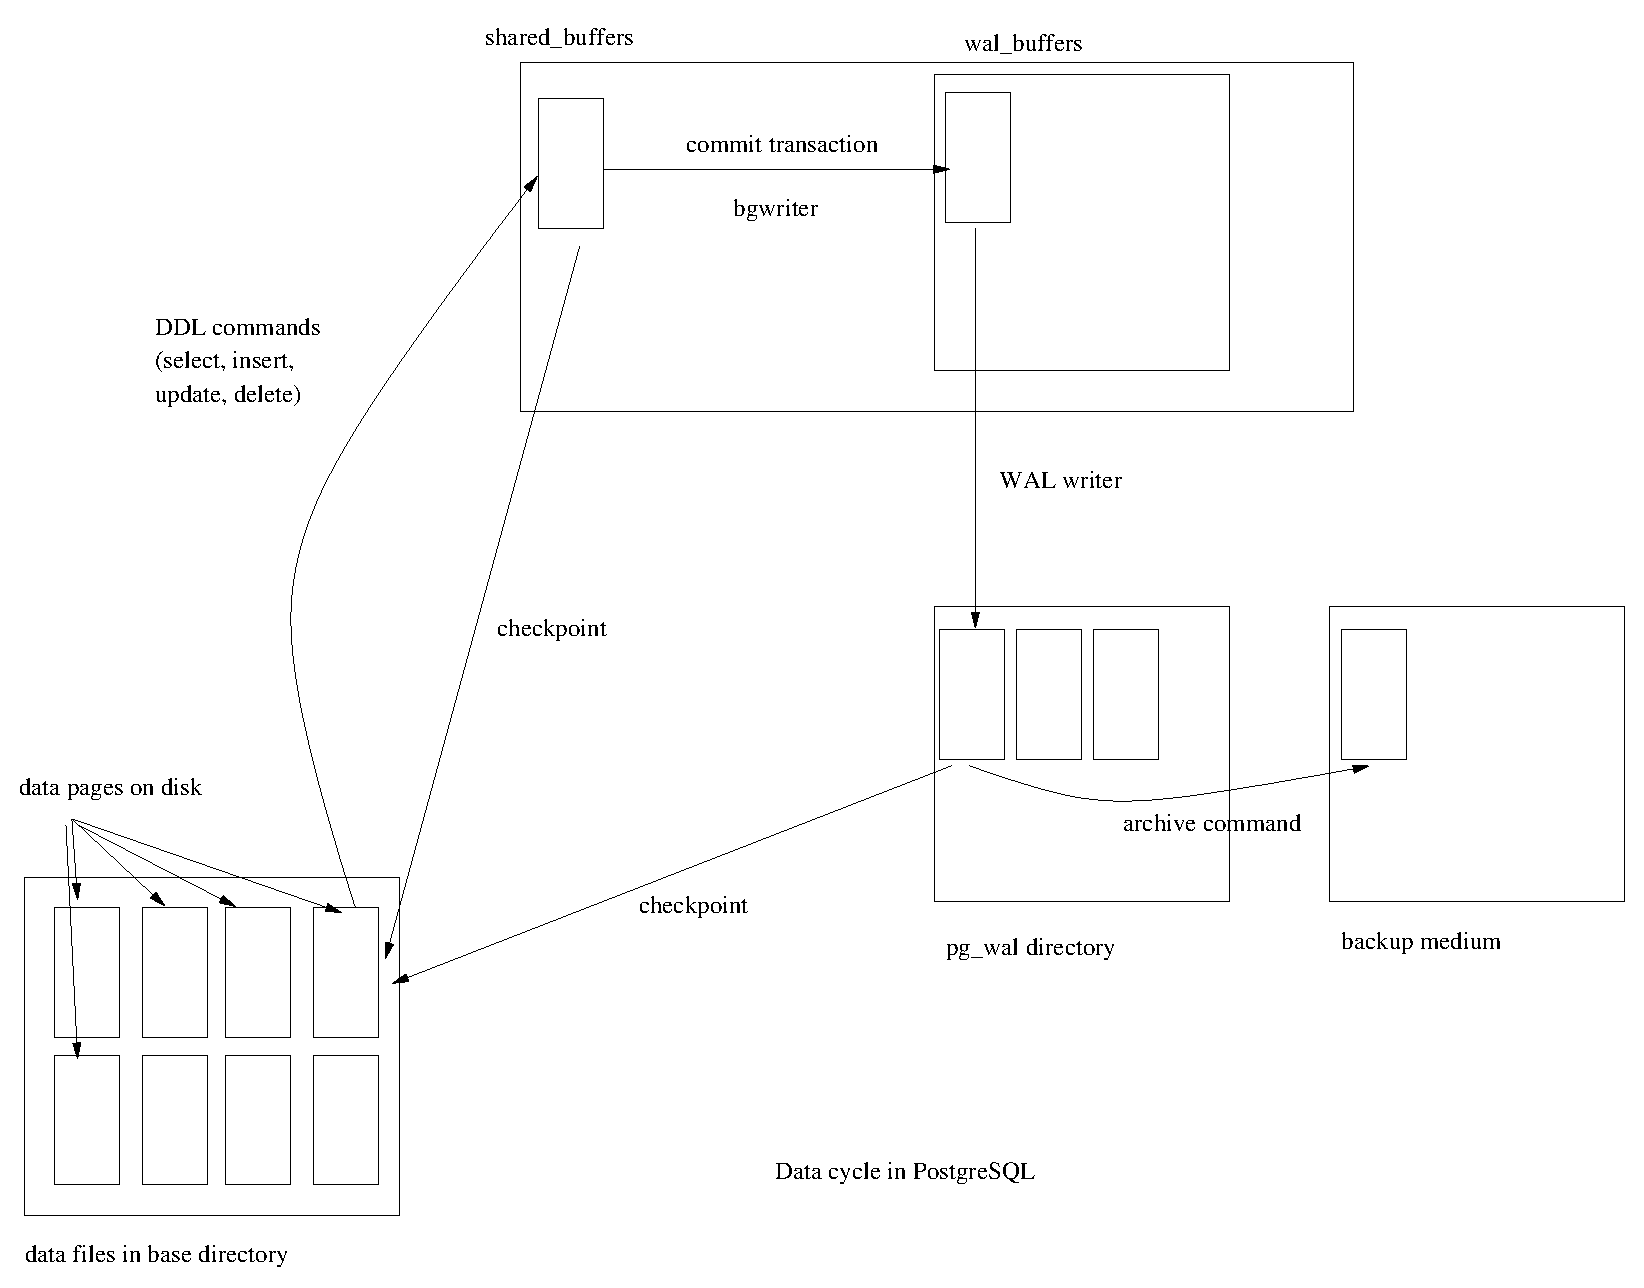
\includegraphics[angle=0, width=0.5\textwidth]{images/internals.eps}
\end{center}
\end{figure}

\begin{toile}
\toileurl{https://www.postgresql.org/docs/15/wal-configuration.html}
\end{toile}

\end{frame}

%%%%%%%%%%%%%%%%%%%%%%%%%%%%%%%%%%%%%%%%%%%%%%%%%%%%%%%%%%%%%%%%%%%%%%%%%%%%%%%%

\begin{frame}{Multiversion Concurrency Control - MVCC}

   \begin{itemize}
      \item PostgreSQL fournit un grand nombre d'outils pour gérer l'accès concurrentiel aux données
      \item De manière interne, la cohérence des données est mise en place en utilisant un modèle multi-versions (MVCC)
      \item Cela signifie que chaque requête SQL a la vision d'un instantané des données (snapshot)
      \item Cet instantané correspond à une version de la base de données il y a quelques instants, quelques soient les modifications actuellement réalisées sur les données
      \item Cela empêche les requêtes de voir des données incohérentes modifiées par des requêtes parallèles
      \item Cette méthode fournit l'isolation transactionnelle pour chaque session de la base des données
   \end{itemize}

\begin{toile}
\toileurl{https://www.postgresql.org/docs/15/mvcc-intro.html}
\end{toile}

\end{frame}

%%%%%%%%%%%%%%%%%%%%%%%%%%%%%%%%%%%%%%%%%%%%%%%%%%%%%%%%%%%%%%%%%%%%%%%%%%%%%%%%

\begin{frame}{Multiversion Concurrency Control - MVCC}

   \begin{itemize}
      \item Le MVCC en évitant les méthodes de verrouillage des bases de données classiques minimise la contention et favorise la performance dans un environnement multi-utilisateurs
      \item En cas de nécessité de verrouillage, il existe différents type de verrous:
      \begin{itemize}
         \item le verrouillage en lecture
         \item le verrouillage en écriture
         \item ces 2 types de verrous ne se gênent pas mutuellement: un verrou en lecture n'empêche pas l'écriture et vice-versa 
      \end{itemize}
   \end{itemize}

\end{frame}

%%%%%%%%%%%%%%%%%%%%%%%%%%%%%%%%%%%%%%%%%%%%%%%%%%%%%%%%%%%%%%%%%%%%%%%%%%%%%%%%

\begin{frame}[fragile]{Mise en place de la génération des WAL}

\begin{itemize}

   \item Pour activer la génération des WAL, merci de modifier les paramètres suivants dans \textit{postgresql.conf}

\begin{intercom}
wal\_level = replica # or higher
archive\_mode = on
[...]
\end{intercom}

\end{itemize}

\begin{toile}
\toileurl{https://www.postgresql.org/docs/15/continuous-archiving.html}
\end{toile}

\end{frame}

%%%%%%%%%%%%%%%%%%%%%%%%%%%%%%%%%%%%%%%%%%%%%%%%%%%%%%%%%%%%%%%%%%%%%%%%%%%%%%%%

\begin{frame}[fragile]{\commande{archive\_command} et \commande{archive\_library}}

\begin{itemize}

   \item La copie des WAL vers le système de sauvegarde se paramètre depuis les 2 valeurs suivantes:

   \begin{itemize}
      \item \textbf{archive\_command}: Commandes shell d'archivage des WAL
      \item \textbf{archive\_library}: Binaire d'archivage des WAL
   \end{itemize}

   \item Chacune des 2 valeurs s'utilise au choix. Elles ne peuvent utilisées en même temps.
   \item Pour les exercices, le paramètre \textbf{archive\_command} sera utilisé.

\begin{tiny}
\begin{Verbatim}[commandchars=\\\{\}]
archive\_command = 'test ! -f /mnt/server/archivedir/\%f && cp \%p /mnt/server/archivedir/\%f' # Unix
   [...]
\end{Verbatim}
\end{tiny}

\end{itemize}

\end{frame}

%%%%%%%%%%%%%%%%%%%%%%%%%%%%%%%%%%%%%%%%%%%%%%%%%%%%%%%%%%%%%%%%%%%%%%%%%%%%%%%%

\begin{frame}[fragile]{Fonctionnement de l'archivage des WAL}

\begin{itemize}

   \item La commande d'archivage des WALs est lancée par le même utilisateur du process \textit{postmaster}
   \item Elle est censée renvoyer un code différent de 0 en cas d'erreur
   \item Il est important de vérifier que le WAL n'existe pas dans le répertoire cible sous peine de l'écraser
   \item En cas d'erreur d'archivage, PostgreSQL retente autant de fois que nécessaire
   \item Tant que le fichier WAL n'est pas archivé, celui-ci n'est pas supprimé du répertoire pg\_wal, ce qui peut amener à une saturation du système de fichiers
   \item En cas de saturation du répertoire pg\_wal, le serveur s'arrête avec une erreur de type PANIC. Il pourra redémarrer une fois qu'il aura de l'espace disque disponible

\end{itemize}

\end{frame}

%%%%%%%%%%%%%%%%%%%%%%%%%%%%%%%%%%%%%%%%%%%%%%%%%%%%%%%%%%%%%%%%%%%%%%%%%%%%%%%%

\begin{frame}[fragile]{Caractéristiques des WAL}

\begin{itemize}

   \item Le nom des fichiers WAL inclut jusqu'à 64 caractères
   \item Il est composé de lettres ASCII, de chiffres et de points
   \item Il est important de garder le nom de l'archive WAL
   \item La sauvegarde des WALs ne permet pas de restaurer \textit{postgresql.conf}, \textit{pg\_hba.conf} ou \textit{pg\_ident.conf}
   \item Il est important de sauvegarder ces 3 fichiers indépendamment
   \item Ces fichiers peuvent être stockés dans un répertoire paramétrable

\end{itemize}

\end{frame}

%%%%%%%%%%%%%%%%%%%%%%%%%%%%%%%%%%%%%%%%%%%%%%%%%%%%%%%%%%%%%%%%%%%%%%%%%%%%%%%%

\begin{frame}[fragile]{Timelines (lignes de temps)}

\begin{itemize}

   \item Après chaque opération de recovery, PostgreSQL créée une nouvelle ligne de temps (timeline)
   \item Au passage, le serveur crée un fichier "timeline history" qui lui indique la série de WAL générés après le recovery
   \item Les WALs créés après l'opération de recovery appartiennent à cette nouvelle ligne de temps
   \item Par défaut, l'opération de recovery rétablit la timeline la plus récente
   \item Il est possible de rétablir une timeline donnée dans le passé


\end{itemize}

\begin{toile}
\toileurl{https://www.postgresql.org/docs/15/continuous-archiving.html}
\end{toile}

\end{frame}


%%%%%%%%%%%%%%%%%%%%%%%%%%%%%%%%%%%%%%%%%%%%%%%%%%%%%%%%%%%%%%%%%%%%%%%%%%%%%%%%

\begin{frame}[fragile]{Format du nom du WAL}

   Dans le répertoire /pg\_wal, on peut voir le WAL suivant:

\begin{itemize}

   \item \textbf{00000001}000000000000001B
   \item La timeline est représentée par les 8 premiers chiffres du nom du WAL

\end{itemize}

\begin{toile}
\toileurl{https://www.postgresql.org/docs/15/continuous-archiving.html}
\end{toile}

\end{frame}


%%%%%%%%%%%%%%%%%%%%%%%%%%%%%%%%%%%%%%%%%%%%%%%%%%%%%%%%%%%%%%%%%%%%%%%%%%%%%%%%

\begin{frame}[fragile]{La commande \commande{pg\_basebackup}}

\begin{itemize}

\item La commande \commande{pg\_basebackup} sauvegarde un cluster PostgreSQL
\item Elle ne s'applique pas sur une base de données en particulier
\item L'utilisateur lançant cette commande doit posséder le droit \textbf{REPLICATION} ou être un super-utilisateur
\item La commande peut être lancée sur un serveur standby
\item La table \textit{pg\_stat\_progress\_basebackup} donne une idée de la progression de la commande

\end{itemize}

\begin{toile}
\toileurl{https://www.postgresql.org/docs/15/app-pgbasebackup.html}
\toileurl{https://www.postgresql.org/docs/15/progress-reporting.html\#BASEBACKUP-PROGRESS-REPORTING}
\end{toile}

\end{frame}

%%%%%%%%%%%%%%%%%%%%%%%%%%%%%%%%%%%%%%%%%%%%%%%%%%%%%%%%%%%%%%%%%%%%%%%%%%%%%%%%

\begin{frame}{Options de la commande \commande{pg\_basebackup}}

   Les options qui semblent les plus intéressantes sont:

\begin{itemize}

   \item \option{-F \textit{format}}
   \item \textit{format} a les valeurs suivantes:
   \begin{itemize}
      \item  \textit{p} ou \textit{plain}. Format par défaut. 
      \item  \textit{t} ou \textit{tar}. Génération d'une archive du répertoire des données \textit{base.tar}
   \end{itemize}

\end{itemize}

\begin{toile}
\toileurl{https://www.postgresql.org/docs/15/app-pgbasebackup.html}
\end{toile}

\end{frame}

%%%%%%%%%%%%%%%%%%%%%%%%%%%%%%%%%%%%%%%%%%%%%%%%%%%%%%%%%%%%%%%%%%%%%%%%%%%%%%%%

\begin{frame}{Options de la commande \commande{pg\_basebackup}}

\begin{itemize}
   \item \option{-R} or \option{{-}{-}write-recovery-conf}
   \begin{itemize}
      \item la commande génère automatiquement le fichier \textbf{standby.signal}
   \end{itemize}
   \item \option{-T \textit{olddir}=\textit{newdir}} ou \option{{-}{-}tablespace-mapping=\textit{olddir}=\textit{newdir}}
   \begin{itemize}
      \item cette option permet de mapper les répertoires du serveur liés aux tablespaces à d'autres répertoires locaux. Option valide uniquement si le format \textbf{plain} est utilisé. 
   \end{itemize}
   \item \option{-X \textit{method}} ou \option{{-}{-}wal-method=\textit{method}}
   \begin{itemize}
   \item \textit{method} a les valeurs suivantes:
      \begin{itemize}
         \item  \textit{n} ou \textit{none}. Le backup n'inclut pas les WAL.
         \item  \textit{f} ou \textit{fetch}. Les WAL générés durant le backup sont récupérés une fois le backup généré. Dans le cas de l'utilisation de cette option, le paramètre \option{wal\_keep\_size} nécessite d'être ajusté correctement afin que le serveur puisse garder l'ensemble des WAL (et ne supprime ni n'en recycle durant le backup).
         \item  \textit{s} ou \textit{stream}. Mode par défaut. Une $2^{\grave{e}me}$ connexion est établie vers le serveur pour streamer les WAL générés durant le backup.
      \end{itemize}
   \end{itemize}
\end{itemize}

\end{frame}

%%%%%%%%%%%%%%%%%%%%%%%%%%%%%%%%%%%%%%%%%%%%%%%%%%%%%%%%%%%%%%%%%%%%%%%%%%%%%%%%

\begin{frame}{Options de la commande \commande{pg\_basebackup}}

\begin{itemize}
   \item \option{{-}{-}no-estimate-size}
   \begin{itemize}
      \item le serveur n'estime plus la taille du backup avant de débuter le process. Cela permet de raccourcir la durée de la génération du backup.
   \end{itemize}

\item{\textbf{Environment}}
   \begin{itemize}
      \item Cet utilitaire, tout comme la majorité des utilitaires PostgreSQL, utilisent les mêmes variables d'environnement que ceux de la libpq.
      \item La variable d'environment PG\_COLOR indique si la couleur est utilisée dans les messages de diagnostique. Les valeurs possibles sont \textsl{always}, \textsl{auto} et \textsl{never}.
   \end{itemize}
\end{itemize}

\end{frame}

%%%%%%%%%%%%%%%%%%%%%%%%%%%%%%%%%%%%%%%%%%%%%%%%%%%%%%%%%%%%%%%%%%%%%%%%%%%%%%%%

\begin{frame}{Checkpoints}
   \label{checkpoint}

\begin{itemize}
   \item A chaque checkpoint, l'ensemble des pages chargées et modifiées (\textsf{dirty pages}) dans les \textsf{shared\_buffers} sont flushées en disque.
   \item Les données présentes dans les WAL sont également écrites en disque.
   \item En cas de rejeu des WAL (\textbf{REDO}), le serveur part de la dernière transaction liée au checkpoint pour rejouer les WALs.
   \item Cette opération engendre une forte activité I/O
   \item La fréquence des checkpoint est liée à 2 paramètres:
   \begin{itemize}
      \item \textbf{checkpoint\_timeout}
      \item \textbf{max\_wal\_size}
   \end{itemize}
\end{itemize}

\begin{toile}
\toileurl{https://www.postgresql.org/docs/current/wal-configuration.html}
\end{toile}

\end{frame}

%%%%%%%%%%%%%%%%%%%%%%%%%%%%%%%%%%%%%%%%%%%%%%%%%%%%%%%%%%%%%%%%%%%%%%%%%%%%%%%%

\begin{frame}{\textbf{checkpoint\_timeout} et \textbf{max\_wal\_size}}

   \textbf{checkpoint\_timeout}
\begin{itemize}
   \item Intervalle en secondes entre 2 checkpoints automatiques
\end{itemize}

   \textbf{max\_wal\_size}
\begin{itemize}
   \item Taille disque maximale occupée par les WAL. Lorsque cette taille est atteinte, l'opération de checkpoint est déclenchée ainsi que \textsf{archive\_command}.
\end{itemize}

   \textbf{min\_wal\_size}
\begin{itemize}
   \item Taille disque minimale occupée par les WAL. Lorsque ce seuil est atteint, les WAL ne sont plus supprimés mais recyclés (renommés).
\end{itemize}

\begin{toile}
\toileurl{https://www.postgresql.org/docs/current/runtime-config-wal.html\#GUC-CHECKPOINT-TIMEOUT}
\toileurl{https://www.postgresql.org/docs/current/runtime-config-wal.html\#GUC-MAX-WAL-SIZE}
\end{toile}

\end{frame}

%%%%%%%%%%%%%%%%%%%%%%%%%%%%%%%%%%%%%%%%%%%%%%%%%%%%%%%%%%%%%%%%%%%%%%%%%%%%%%%%

\begin{frame}[fragile]{La commande \commande{pg\_verifybackup}}

\begin{itemize}

   \item La commande \commande{pg\_verifybackup} vérifie l'intégrité d'une sauvegarde générée par la commande \commande{pg\_basebackup}
   \item Elle s'applique sur un backup généré au format plain. Dans le cas de la vérification d'une archive tar, il est nécessaire de désarchiver auparavant.

\end{itemize}

\begin{toile}
\toileurl{https://www.postgresql.org/docs/15/app-pgverifybackup.html}
\end{toile}

\end{frame}

%%%%%%%%%%%%%%%%%%%%%%%%%%%%%%%%%%%%%%%%%%%%%%%%%%%%%%%%%%%%%%%%%%%%%%%%%%%%%%%%

\begin{frame}[fragile]{La commande \commande{pg\_amcheck}}

\begin{itemize}

   \item La commande \commande{pg\_amcheck} vérifie l'intégrité d'une base de données.
   \item Fait appel à l'utilitaire \textsf{amcheck}
   \item S'applique aux tables ordinaires, celles de type TOAST, les vues matérialisées, les séquences, les indexes btree.
   \item Possède des options de filtrages de base, de schéma et de table

\end{itemize}

\begin{toile}
\toileurl{https://www.postgresql.org/docs/current/app-pgamcheck.html}
\toileurl{https://www.postgresql.org/docs/current/amcheck.html}
\end{toile}

\end{frame}

%%%%%%%%%%%%%%%%%%%%%%%%%%%%%%%%%%%%%%%%%%%%%%%%%%%%%%%%%%%%%%%%%%%%%%%%%%%%%%%%

\begin{frame}[fragile]{Principales options de la commande \commande{pg\_amcheck}}

   Les principales options de cette commande sont:

\begin{itemize}

   \item \option{{-}{-}no-dependent-indexes} exclut de la vérification les indexes associés à la table
   \item \option{{-}{-}no-dependent-toast} exclut de la vérification les tables TOAST associées à la table
   \item Options applicables aux indexes

   \begin{itemize}
      \item \option{{-}{-}heapallindexed} crée un nouvel index temporaire en mémoire pour vérifier que l'index actuellement stocké est valide. Cette option utilise de la RAM limitée par le paramètre \option{maintenance\_work\_mem}
   \end{itemize}
\end{itemize}

\end{frame}

%%%%%%%%%%%%%%%%%%%%%%%%%%%%%%%%%%%%%%%%%%%%%%%%%%%%%%%%%%%%%%%%%%%%%%%%%%%%%%%%

\begin{frame}{Options de la commande \commande{pg\_amcheck}}

\begin{itemize}
   \item \option{{-}{-}parent-check} vérifie les indexes de la table parent\footnote{https://www.postgresql.org/docs/current/ddl-inherit.html}
\end{itemize}

\end{frame}

%%%%%%%%%%%%%%%%%%%%%%%%%%%%%%%%%%%%%%%%%%%%%%%%%%%%%%%%%%%%%%%%%%%%%%%%%%%%%%%%

\section{Exercice}

%%%%%%%%%%%%%%%%%%%%%%%%%%%%%%%%%%%%%%%%%%%%%%%%%%%%%%%%%%%%%%%%%%%%%%%%%%%%%%%%

\begin{frame}{Réalisation d'un backup full de la base de données}

La procédure de déroulement du PITR s'appuie sur:
\begin{itemize}
   \item la génération d'un backup full
   \item l'archivage des WALs
\end{itemize}


Il existe 2 méthodes pour réaliser une sauvegarde full de la base données:
\begin{itemize}
   \item l'outil \textsf{pg\_basebackup}
   \item l'API bas niveau avec des appels aux fonctions PostgreSQL
\end{itemize}

La méthode étudiée pendant les exercices est l'outil \textsf{pg\_basebackup}.

\end{frame}

%%%%%%%%%%%%%%%%%%%%%%%%%%%%%%%%%%%%%%%%%%%%%%%%%%%%%%%%%%%%%%%%%%%%%%%%%%%%%%%%

\begin{frame}[fragile]\frametitle{Mise en place de l'archivage des WALs}

\begin{itemize}
   \item Vérifier que PostgreSQL est déployé sur les serveurs \textsf{hqpg-0x} et \textsf{hqpg-0x-repl}
   \item Mettre en place la copie des WAL vers le répertoire \path{/opt/wal_backup} avec le niveau \textbf{replica}
   \item La commande \textsf{archive\_command} s'appuie sur rsync pour transférer les WALs depuis le primaire. Pour éviter d'avoir à indiquer le mot de l'utilisateur postgres, réaliser la génération et l'échange mutuel de clefs SSH sur les 2 serveurs comme décrit en page ~\ref{sec:ssh-keys}
   \item Paramétrer la commande \textsf{archive\_command} dans postgresql.conf
   \begin{tiny}
      \item \commande{archive\_command = 'rsync \%p hqpg-0x-repl:/opt/wal\_backup/\%f'}
   \end{tiny}

\end{itemize}

\end{frame}

%%%%%%%%%%%%%%%%%%%%%%%%%%%%%%%%%%%%%%%%%%%%%%%%%%%%%%%%%%%%%%%%%%%%%%%%%%%%%%%%

\begin{frame}[fragile]\frametitle{Résumé du paramétrage de la sauvegarde des WALs}

Sur le serveur principal, les lignes suivantes sont inclues dans postgresql.conf:
\begin{tiny}
\begin{verbatim}
# Add settings for extensions here
listen_addresses = '*'
wal_level = replica
archive_mode = on
archive_command = 'rsync %p 10.10.10.29:/opt/archivedir/%f'
\end{verbatim}
\end{tiny}

\begin{itemize}
   \item Sur le serveur de sauvegarde, créer le répertoire \path{/opt/wal_backup/} de sauvegarde des WALs avec l'utilisateur postgres
\end{itemize}

\end{frame}

%%%%%%%%%%%%%%%%%%%%%%%%%%%%%%%%%%%%%%%%%%%%%%%%%%%%%%%%%%%%%%%%%%%%%%%%%%%%%%%%

\begin{frame}[fragile]\frametitle{Remarque importante sur la procédure de PITR}

\begin{small}
   \textbf{Remarque} Le point de restauration est obligatoirement après la date de fin du base backup, c'est à dire, le temps de fin de l'appel à pg\_basebackup\_stop. Il n'est possible de restaurer des données à une date durant laquelle le backup est en cours.
Pour restaurer à une telle date, il est nécessaire de restaurer le précédent backup et de rejouer les sauvegardes WALs jusqu'à ce point.
\end{small}

\end{frame}

%%%%%%%%%%%%%%%%%%%%%%%%%%%%%%%%%%%%%%%%%%%%%%%%%%%%%%%%%%%%%%%%%%%%%%%%%%%%%%%%

\begin{frame}[fragile]\frametitle{Utilisation de \textsf{pg\_basebackup} pour sauvegarder la base de données}

Sur le serveur principal, ajouter la ligne suivante dans pg\_hba.conf:

\begin{tiny}
\begin{Verbatim}[commandchars=\\\{\}]
host  replication  postgres   10.10.10.0/24  trust
\end{Verbatim}
\end{tiny}

Recharger le paramétrage avec la commande suivante:

\begin{tiny}
\begin{verbatim}
postgres=# SELECT pg_reload_conf();
\end{verbatim}
\end{tiny}

\end{frame}

%%%%%%%%%%%%%%%%%%%%%%%%%%%%%%%%%%%%%%%%%%%%%%%%%%%%%%%%%%%%%%%%%%%%%%%%%%%%%%%%

\begin{frame}[fragile]\frametitle{Génération d'un backup full}

Sur le serveur de sauvegarde des WAL, appliquer les commandes suivantes:

\begin{itemize}
   \item Comme indiqué dans\footnote{https://www.postgresql.org/docs/current/app-pgbasebackup.html}, la commande \textsf{pg\_basebackup} réalise un checkpoint (p. \ref{checkpoint}) sur le serveur
   \item \commande{pg\_basebackup -h hqpg-0x -Ft -z -P -D /opt/backup/20230213}
\end{itemize}

\end{frame}

%%%%%%%%%%%%%%%%%%%%%%%%%%%%%%%%%%%%%%%%%%%%%%%%%%%%%%%%%%%%%%%%%%%%%%%%%%%%%%%%

\begin{frame}[fragile]\frametitle{Inspection de l'archive générée}

\begin{tiny}
\begin{verbatim}
[postgres@localhost 20230202_1]$ ls -lrt
total 4420
-rw------- 1 postgres postgres  181880  2 févr. 07:58 backup_manifest
-rw------- 1 postgres postgres 4321056  2 févr. 07:58 base.tar.gz
-rw------- 1 postgres postgres   17075  2 févr. 07:58 pg_wal.tar.gz
\end{verbatim}
\end{tiny}

\begin{itemize}
   \item backup\_manifest inclut le listing avec les checkum de l'archive base.tar.gz
   \item pg\_wal.tar.gz inclut les WAL générés durant l'opération du pg\_basebackup
\end{itemize}

\end{frame}

%%%%%%%%%%%%%%%%%%%%%%%%%%%%%%%%%%%%%%%%%%%%%%%%%%%%%%%%%%%%%%%%%%%%%%%%%%%%%%%%

\begin{frame}[fragile]\frametitle{Création du jeu de données}

Sur le serveur principal, lancer les commandes suivantes:

\begin{tiny}
\begin{verbatim}
su - postgres
creatuser hq -d
createdb hqdb -O hq
psql hqdb
-- 02/02/2023 16h27
create table test_pitr1 (col1 text);
create table test_pitr2 (col1 text);
-- quelques minutes plus tard
-- 16h30
create table test_pitr3 (col1 text);
\end{verbatim}
\end{tiny}

\begin{toile}
\toileurl{https://www.postgresql.org/docs/current/app-createuser.html}
\toileurl{https://www.postgresql.org/docs/current/app-createdb.html}
\end{toile}


\end{frame}

%%%%%%%%%%%%%%%%%%%%%%%%%%%%%%%%%%%%%%%%%%%%%%%%%%%%%%%%%%%%%%%%%%%%%%%%%%%%%%%%

\begin{frame}[fragile]\frametitle{Restauration de la base de données à une date donnée}

Sur le serveur PostgreSQL principal,

\begin{tiny}
\begin{verbatim}
[root@localhost 15]# systemctl stop postgresql-15.service
[root@localhost 15]# su - postgres
Dernière connexion : samedi  4 février 2023 à 20:01:48 EST sur pts/0
[postgres@localhost ~]$ cd 15
# mv data data.20230213
# scp 10.10.10.29:/opt/backup/20230205_1/* .
# rm -rf data && mkdir data && chmod 0700 data
# tar xvzf ../base.tar.gz 
# cd pg_wal/
# tar xvzf ../../pg_wal.tar.gz 
#  cd ..
#  touch recovery.signal
\end{verbatim}
\end{tiny}

\begin{toile}
\toileurl{https://www.postgresql.org/docs/15/runtime-config-wal.html\#RUNTIME-CONFIG-WAL-RECOVERY-TARGET}
\end{toile}

\end{frame}

%%%%%%%%%%%%%%%%%%%%%%%%%%%%%%%%%%%%%%%%%%%%%%%%%%%%%%%%%%%%%%%%%%%%%%%%%%%%%%%%

\begin{frame}[fragile]\frametitle{Restauration de la base de données à une date donnée}

Ajouter les lignes suivantes dans postgresql.conf

\begin{tiny}
\begin{verbatim}
restore_command = 'rsync 10.10.10.29:/opt/archivedir/%f %p'
recovery_target_time = '2023-02-05 02:20:00+01'
\end{verbatim}
\end{tiny}

Démarrer le serveur avec la commande.

\end{frame}

%%%%%%%%%%%%%%%%%%%%%%%%%%%%%%%%%%%%%%%%%%%%%%%%%%%%%%%%%%%%%%%%%%%%%%%%%%%%%%%%

\begin{frame}[fragile]\frametitle{Logs de la restauration}

\begin{tiny}
\begin{Verbatim}[commandchars=\\\{\}]
rsync: link_stat "/opt/archivedir/00000002.history" failed: No such file or directory (2)
rsync error: some files/attrs were not transferred (see previous errors) (code 23) at main.c(1670) [Receiver=3.1.3]
2023-02-04 20:28:02.203 EST [22385] LOG:  début de la restauration de l'archive à \userinput{2023-02-04 20:20:00-05}
2023-02-04 20:28:03.278 EST [22385] LOG:  la ré-exécution commence à 0/1C000028
2023-02-04 20:28:03.648 EST [22385] LOG:  restauration du journal de transactions « 00000001000000000000001D » à partir de l'archive
2023-02-04 20:28:05.011 EST [22385] LOG:  état de restauration cohérent atteint à 0/1C000100
2023-02-04 20:28:05.011 EST [22381] LOG:  le système de bases de données est prêt pour accepter les connexions en lecture seule
rsync: link_stat "/opt/archivedir/00000001000000000000001F" failed: No such file or directory (2)
2023-02-04 20:28:05.172 EST [22385] LOG:  arrêt de la restauration avant validation de la transaction 740, 2023-02-04 20:21:11.941687-05
2023-02-04 20:28:05.172 EST [22385] LOG:  pause à la fin de la restauration
2023-02-04 20:28:05.172 EST [22385] \userinput{ASTUCE :  Exécuter pg_wal_replay_resume() pour promouvoir.}
2023-02-04 20:33:01.702 EST [22383] LOG:  début du restartpoint : time
2023-02-04 20:33:05.828 EST [22383] LOG:  restartpoint terminé : a écrit 26 tampons (0.2%); 0 fichiers WAL ajoutés, 2 supprimés, 0 recyclés ; écriture=3.090 s, synchronisation=0.610 s, total=4.127 s; fichiers synchronisés=18, plus long=0.609 s, moyenne=0.034 s; distance=32768 kB, estimation=32768 kB
2023-02-04 20:33:05.829 EST [22383] LOG:  la ré-exécution en restauration commence à 0/1E000028
\end{Verbatim}
\end{tiny}

\end{frame}

%%%%%%%%%%%%%%%%%%%%%%%%%%%%%%%%%%%%%%%%%%%%%%%%%%%%%%%%%%%%%%%%%%%%%%%%%%%%%%%%

\begin{frame}[fragile]\frametitle{Basculement de la base de données en mode écriture}

\begin{tiny}
\begin{verbatim}
hqdb=# create table test_pitr_20230206144000 (col1 text);
ERREUR:  ne peut pas exécuter CREATE TABLE dans une transaction en lecture seule
hqdb=# quit
[postgres@localhost pg_wal]$ psql
psql (15.1)
Saisissez « help » pour l'aide.

postgres=# select pg_wal_replay_resume();
 pg_wal_replay_resume 
----------------------
 
(1 ligne)

postgres=# create table test_pitr_20230206144000 (col1 text);
CREATE TABLE
\end{verbatim}
\end{tiny}

\end{frame}

%%%%%%%%%%%%%%%%%%%%%%%%%%%%%%%%%%%%%%%%%%%%%%%%%%%%%%%%%%%%%%%%%%%%%%%%%%%%%%%%

\begin{frame}[fragile]\frametitle{Apparition d'une nouvelle ligne de temps}

\begin{tiny}
\begin{Verbatim}[commandchars=\\\{\}]
[postgres@localhost pg_wal]$ ls -lrt
total 32772
-rw------- 1 postgres postgres 16777216  6 févr. 08:41 00000001000000000000001E
\userinput{-rw------- 1 postgres postgres       51  6 févr. 08:41 00000002.history}
drwx------ 2 postgres postgres       72  6 févr. 08:41 archive_status
\userinput{-rw------- 1 postgres postgres 16777216  6 févr. 08:46 00000002000000000000001E}
\end{Verbatim}
\end{tiny}

\end{frame}

%%%%%%%%%%%%%%%%%%%%%%%%%%%%%%%%%%%%%%%%%%%%%%%%%%%%%%%%%%%%%%%%%%%%%%%%%%%%%%%%

\begin{frame}[fragile]\frametitle{Génération et échange mutuel des clés SSH}
\label{sec:ssh-keys}

\begin{tiny}
\begin{verbatim}
[linagora@localhost ~]$ sudo -i
[root@localhost ~]# su - postgres
[postgres@localhost ~]$ ssh-keygen 
Generating public/private rsa key pair.
Enter file in which to save the key (/var/lib/pgsql/.ssh/id_rsa): 
Enter passphrase (empty for no passphrase): 
Enter same passphrase again: 
\end{verbatim}
\end{tiny}

\begin{itemize}
   \item Copier la clef publique dans le répertoire $\sim/postgres/.ssh/authorized\_keys$
   \item Vérifier avec la commande ssh \textsf{postgres@hqpg-0x-repl} et inversement que la session SSH est établie sans avoir à fournir de mot de passe
\end{itemize}

\end{frame}

%%%%%%%%%%%%%%%%%%%%%%%%%%%%%%%%%%%%%%%%%%%%%%%%%%%%%%%%%%%%%%%%%%%%%%%%%%%%%%%%

\begin{frame}[fragile]{En cas de corruption des WALs}

\begin{itemize}

   \item Dans le cas où l'opération de recovery détecte un WAL corrompu, l'opération s'interompt et le serveur ne démarre pas. Il est possible de relancer l'opération de recovery avec une cible de recovery située avant le point de corruption pour permettre à l'opération de se terminer.
   \item Dans le cas où l'opération de recovery échoue pour une raison externe (crash système ou archive WAL inaccessible), le recovery peut être relancera. Il reprendra proche du point où il s'est interrompu.
   \item Le redémarrage du mode recovery fonctionne de manière similaire au checkpoint en mode normal: le serveur enregistre son état de manière périodique en disque, puis met à jour le fichier pg\_control pour indiquer les WAL déjà traités et qui ne nécessitent pas d'être scannées à nouveau.
\end{itemize}

\begin{toile}
\toileurl{https://www.postgresql.org/docs/15/continuous-archiving.html}
\end{toile}

\end{frame}

%%%%%%%%%%%%%%%%%%%%%%%%%%%%%%%%%%%%%%%%%%%%%%%%%%%%%%%%%%%%%%%%%%%%%%%%%%%%%%%%

\begin{frame}[fragile]{Modèles de base de données - Template databases}

\begin{itemize}
   \item La commande \textbf{CREATE DATABASE} fonctionne en copiant une base de données.
   \item Par défaut, elle copie la base de données standard \textbf{template1}.
   \item Si des objets sont créés dans template1, ils seront présents dans les bases créées ultérieurement
   \item Par exemple, si le langage PL/Perl est déployé sur template1, il sera présent sur l'ensemble des bases dérivées
\end{itemize}

\begin{toile}
\toileurl{https://www.postgresql.org/docs/15/manage-ag-templatedbs.html}
\end{toile}

\end{frame}



%%%%%%%%%%%%%%%%%%%%%%%%%%%%%%%%%%%%%%%%%%%%%%%%%%%%%%%%%%%%%%%%%%%%%%%%%%%%%%%%

\subsection{Supervision des processus de la base de données}

%%%%%%%%%%%%%%%%%%%%%%%%%%%%%%%%%%%%%%%%%%%%%%%%%%%%%%%%%%%%%%%%%%%%%%%%%%%%%%%%

\begin{frame}[fragile]{Supervision de la base de données}

   TODO
   WIP

\begin{toile}
\toileurl{https://www.postgresql.org/docs/15/monitoring.html}
\end{toile}

\end{frame}

%%%%%%%%%%%%%%%%%%%%%%%%%%%%%%%%%%%%%%%%%%%%%%%%%%%%%%%%%%%%%%%%%%%%%%%%%%%%%%%%

\begin{frame}{L'importance des sauvegardes}

\begin{itemize}

\item Il est important de posséder 2 copies supplémentaires à la copie des données de productions.
\item Une des 2 copies se situe hors site.
\item Chacune des 2 copies est stockée sur un média différent.

\end{itemize}

\begin{toile}
\toileurl{https://www.it-connect.fr/sauvegarde-quest-ce-que-la-regle-du-3-2-1/}
\end{toile}

\end{frame}

%%%%%%%%%%%%%%%%%%%%%%%%%%%%%%%%%%%%%%%%%%%%%%%%%%%%%%%%%%%%%%%%%%%%%%%%%%%%%%%%

\begin{frame}[fragile]{Différents types de sauvegardes}

Il existe différents types de sauvegarde:

\begin{itemize}

   \item logique avec les commandes \commande{pg\_dump} et \commande{pg\_dumpall}
   \item au niveau du système de fichiers avec la commande \commande{tar}.\footnote{La sauvegarde du système de fichiers n'est pas recommandée par la documentation officielle de PostgreSQL}
   \item binaire avec la commande \commande{pg\_basebackup}

\end{itemize}

\begin{toile}
\toileurl{https://www.postgresql.org/docs/15/backup.html}
\end{toile}

\end{frame}

%%%%%%%%%%%%%%%%%%%%%%%%%%%%%%%%%%%%%%%%%%%%%%%%%%%%%%%%%%%%%%%%%%%%%%%%%%%%%%%%

\begin{frame}[fragile]{Mise en place de la génération des WAL (1/2)}

\begin{itemize}

   \item Pour activer la génération des WAL, merci de modifier les paramètres suivants dans \textit{postgresql.conf}

\begin{intercom}
wal\_level = replica # or higher
archive\_mode = on
[...]
\end{intercom}

\end{itemize}

\begin{toile}
\toileurl{https://www.postgresql.org/docs/15/continuous-archiving.html}
\end{toile}

\end{frame}

%%%%%%%%%%%%%%%%%%%%%%%%%%%%%%%%%%%%%%%%%%%%%%%%%%%%%%%%%%%%%%%%%%%%%%%%%%%%%%%%

\begin{frame}[fragile]{\commande{archive\_command} et \commande{archive\_library}}

\begin{itemize}

   \item La copie des WAL vers le système de sauvegarde se paramètre depuis les 2 valeurs suivantes:

   \begin{itemize}
      \item \textbf{archive\_command}: Commandes shell d'archivage des WAL
      \item \textbf{archive\_library}: Binaire d'archivage des WAL
   \end{itemize}

   \item Chacune des 2 valeur s'utilise au choix. Elles ne peuvent utilisées en même temps.
   \item Pour les exercices, le paramètre \textbf{archive\_command} sera utilisé.

\begin{scriptsize}
   \begin{intercom}
archive\_command = 'test ! -f /mnt/server/archivedir/\%f && cp \%p /mnt/server/archivedir/\%f' # Unix
   [...]
   \end{intercom}
\end{scriptsize}

\end{itemize}

\end{frame}

%%%%%%%%%%%%%%%%%%%%%%%%%%%%%%%%%%%%%%%%%%%%%%%%%%%%%%%%%%%%%%%%%%%%%%%%%%%%%%%%

\begin{frame}[fragile]{Fonctionnement de l'archivage des WAL}

\begin{itemize}

   \item La commande d'archivage des WALs est lancée par le même utilisateur du process \textit{postmaster}
   \item Elle est censée renvoyer un code différent de 0 en cas d'erreur
   \item Il est important de vérifier que le WAL n'existe pas dans le répertoire cible sous peine de l'écraser
   \item En cas d'erreur d'archivage, PostgreSQL retente autant de fois que nécessaire
   \item Tant que le fichier WAL n'est pas archivé, celui-ci n'est pas supprimé du répertoire pg\_wal, ce qui peut amener à une saturation du système de fichiers
   \item En cas de saturation du répertoire pg\_wal, le serveur s'arrête avec une erreur de type PANIC. Il pourra redémarrer une fois qu'il aura de l'espace disque disponible

\end{itemize}

\end{frame}

%%%%%%%%%%%%%%%%%%%%%%%%%%%%%%%%%%%%%%%%%%%%%%%%%%%%%%%%%%%%%%%%%%%%%%%%%%%%%%%%

\begin{frame}[fragile]{Caractéristique des WAL}

\begin{itemize}

   \item Le nom des fichiers WAL inclut jusqu'à 64 caractères
   \item Il est composé de lettres ASCII, de chiffres et de points
   \item Il est important de garder le nom de l'archive WAL
   \item La sauvegarde des WALs ne permet pas de restaurer \textit{postgresql.conf}, \textit{pg\_hba.conf} ou \textit{pg\_ident.conf}
   \item Il est important de sauvegarder ces 3 fichiers indépendamment
   \item Ces fichiers peuvent être stockés dans un répertoire paramétrable

\end{itemize}

\end{frame}

%%%%%%%%%%%%%%%%%%%%%%%%%%%%%%%%%%%%%%%%%%%%%%%%%%%%%%%%%%%%%%%%%%%%%%%%%%%%%%%%

\begin{frame}[fragile]{La commande \commande{pg\_basebackup}}

\begin{itemize}

\item La commande \commande{pg\_basebackup} sauvegarde un cluster PostgreSQL
\item Elle ne s'applique sur une base de données en particulier
\item L'utilisateur lançant cette commande doit posséder le droit \textbf{REPLICATION} ou être un super-utilisateur
\item La commande peut être lancée sur un serveur standby
\item La table \textit{pg\_stat\_progress\_basebackup} donne une idée de la progression de la commande

\end{itemize}

\begin{toile}
\toileurl{https://www.postgresql.org/docs/15/app-pgbasebackup.html}
\toileurl{https://www.postgresql.org/docs/15/progress-reporting.html\#BASEBACKUP-PROGRESS-REPORTING}
\end{toile}

\end{frame}

%%%%%%%%%%%%%%%%%%%%%%%%%%%%%%%%%%%%%%%%%%%%%%%%%%%%%%%%%%%%%%%%%%%%%%%%%%%%%%%%

\begin{frame}{\path{/dev}}

\begin{itemize}

\item Le pseudo-système de fichiers \path{/dev} contient les fichiers spéciaux
permettant l'accès au matériel.

\item Ces fichiers spéciaux sont adaptés au matériel détecté par le noyau lors
de son démarrage et les fichiers idoines sont créés ou supprimés dynamiquement
par la suite en fonction du branchement ou du débranchement de périphériques.

\item C'est un système nommé « udev », dont le fonctionnement est réparti entre
le noyau et un daemon, qui gère le pseudo-système de fichiers \path{/dev}. Il
est au programme de l'examen 201.

\end{itemize}

\begin{toile}
\toileurl{http://fr.wikipedia.org/wiki/Udev}
\end{toile}

\end{frame}

%%%%%%%%%%%%%%%%%%%%%%%%%%%%%%%%%%%%%%%%%%%%%%%%%%%%%%%%%%%%%%%%%%%%%%%%%%%%%%%%

\begin{frame}{\path{/proc}}

\begin{itemize}

\item Le pseudo-système de fichiers \path{/proc} contient :

	\begin{itemize}

	\item un répertoire par processus, nommé selon son PID

	\item un lien symbolique \path{self} pointant vers le répertoire
	correspondant au processus courant

	\item divers fichiers contenant des informations générales, par
	exemple :

\bigskip

\begin{tabulary}{\largeurtableau}{lJ}
\hline
\path{/proc/cmdline}	& paramètres passés au noyau par le chargeur
				d'amorçage		\\
\path{/proc/cpuinfo}	& microprocesseur(s)		\\
\path{/proc/interrupts}	& interruptions			\\
\path{/proc/loadavg}	& charge moyenne		\\
\path{/proc/meminfo}	& utilisation de la mémoire	\\
\hline
\end{tabulary}

	\end{itemize}

\end{itemize}

\begin{toile}
\toileurl{http://fr.wikipedia.org/wiki/Procfs}
\end{toile}

\end{frame}

%%%%%%%%%%%%%%%%%%%%%%%%%%%%%%%%%%%%%%%%%%%%%%%%%%%%%%%%%%%%%%%%%%%%%%%%%%%%%%%%

\begin{frame}[fragile]{\path{/sys}}

\begin{itemize}

\item Le pseudo-système de fichiers \path{/sys} fournit de nombreuses
informations concernant le matériel et les pilotes.

\item Exemple :

\begin{intercom}
\$ cat /sys/class/net/eth0/address
00:1c:23:30:20:13
\end{intercom}

\end{itemize}

\begin{toile}
\toileurl{http://fr.wikipedia.org/wiki/Sysfs}
\end{toile}

\end{frame}

%%%%%%%%%%%%%%%%%%%%%%%%%%%%%%%%%%%%%%%%%%%%%%%%%%%%%%%%%%%%%%%%%%%%%%%%%%%%%%%%

\subsection{Démarrage du système}

%%%%%%%%%%%%%%%%%%%%%%%%%%%%%%%%%%%%%%%%%%%%%%%%%%%%%%%%%%%%%%%%%%%%%%%%%%%%%%%%

% TODO démarrage single user

%%%%%%%%%%%%%%%%%%%%%%%%%%%%%%%%%%%%%%%%%%%%%%%%%%%%%%%%%%%%%%%%%%%%%%%%%%%%%%%%

% TODO Provide common commands to the boot loader and options to the kernel at boot time.
% TODO Demonstrate knowledge of the boot sequence from BIOS to boot completion.
% TODO Check boot events in the log files.

% TODO /var/log/messages

%%%%%%%%%%%%%%%%%%%%%%%%%%%%%%%%%%%%%%%%%%%%%%%%%%%%%%%%%%%%%%%%%%%%%%%%%%%%%%%%

\subsection{Changement de niveaux d'exécution et arrêt ou redémarrage du système}

%%%%%%%%%%%%%%%%%%%%%%%%%%%%%%%%%%%%%%%%%%%%%%%%%%%%%%%%%%%%%%%%%%%%%%%%%%%%%%%%

\begin{frame}{Les commandes \commande{halt}, \commande{poweroff} et
\commande{reboot}}

\begin{itemize}

\item Équivalentes à la commande \commande{shutdown} utilisée avec certaines
options :

\bigskip

\begin{tabular}{|l|l|}
\hline
\commande{halt}		& \commande{shutdown} \option{-H}	\\
\hline
\commande{poweroff}	& \commande{shutdown} \option{-P}	\\
\hline
\commande{reboot}	& \commande{shutdown} \option{-r}	\\
\hline
\end{tabular}

\bigskip

\item Contrairement à \commande{shutdown}, ces commandes ne permettent
d'indiquer ni de délai (elles ont un effet immédiat) ni de message pour les
utilisateurs connectés.

\end{itemize}

\begin{toile}
\toileurl{http://fr.wikipedia.org/wiki/Halt}
\end{toile}

\end{frame}

%%%%%%%%%%%%%%%%%%%%%%%%%%%%%%%%%%%%%%%%%%%%%%%%%%%%%%%%%%%%%%%%%%%%%%%%%%%%%%%%

% TODO Knowledge of basic features of systemd and Upstart.


%%%%%%%%%%%%%%%%%%%%%%%%%%%%%%%%%%%%%%%%%%%%%%%%%%%%%%%%%%%%%%%%%%%%%%%%%%%%%%%%

\begin{frame}{L'examen 101}

\begin{itemize}

\item Dure 1 h 30.

\item Comprend 60 questions.

\item Le score maximum est de 800.

\item Un score de 500 est nécessaire pour réussir l'examen.

\item C'est-à-dire 62,5 \% du score maximum soit environ 37,5 questions.

\end{itemize}

\begin{toile}
\toileurl{http://www.lpi.org/linux-certifications/programs/lpic-1/exam-101/}
\toileurl{http://wiki.lpi.org/wiki/LPIC-1_Objectives(FR)\#Objectifs_de_l.27examen_LPI_101}
\end{toile}

\end{frame}

%%%%%%%%%%%%%%%%%%%%%%%%%%%%%%%%%%%%%%%%%%%%%%%%%%%%%%%%%%%%%%%%%%%%%%%%%%%%%%%%

\section*{Bibliographie}

\pdfbookmark[2]{Bibliographie}{bibliographie}

%%%%%%%%%%%%%%%%%%%%%%%%%%%%%%%%%%%%%%%%%%%%%%%%%%%%%%%%%%%%%%%%%%%%%%%%%%%%%%%%

\section*{Webographie}

\pdfbookmark[2]{Webographie}{webographie}


%%%%%%%%%%%%%%%%%%%%%%%%%%%%%%%%%%%%%%%%%%%%%%%%%%%%%%%%%%%%%%%%%%%%%%%%%%%%%%%%


%%%%%%%%%%%%%%%%%%%%%%%%%%%%%%%%%%%%%%%%%%%%%%%%%%%%%%%%%%%%%%%%%%%%%%%%%%%%%%%%

\section*{Sommaire}

\pdfbookmark[2]{Sommaire}{sommaire}

\begin{frame}{Sommaire}

\tableofcontents[hideallsubsections]

\end{frame}

%%%%%%%%%%%%%%%%%%%%%%%%%%%%%%%%%%%%%%%%%%%%%%%%%%%%%%%%%%%%%%%%%%%%%%%%%%%%%%%%

\section*{Conclusion}

\pdfbookmark[2]{Conclusion}{conclusion}

%\merci

%%%%%%%%%%%%%%%%%%%%%%%%%%%%%%%%%%%%%%%%%%%%%%%%%%%%%%%%%%%%%%%%%%%%%%%%%%%%%%%%

\end{document}
